\section{Geometric Constraints}

\begin{frame}{The Starting Point: Roots in Euclidean Space}
    \textbf{Assumed Structure:} Let $\mathfrak{g}$ be a complex semi-simple Lie algebra.
    We assume the Cartan-Weyl decomposition:
    $$ \mathfrak{g} = \mathfrak{h} \oplus \bigoplus_{\alpha \in \mathcal{R}} \mathfrak{g}_\alpha $$

    % VOCAL CUE: Dichiara a voce che la Forma di Killing induce un prodotto scalare definito positivo su E.
    The roots $\alpha \in \mathcal{R}$ live in a real Euclidean space $E = \mathfrak{h}_{\mathbb{R}}^\vee$, equipped with a scalar product $(\cdot, \cdot)$ inherited from the Killing form.

    \vspace{0.3cm}
    \textbf{Physical Meaning:} The roots represent the gauge bosons (like $W^\pm$, gluons) that mediate transitions between quantum states charged under the Cartan generators.

    \vfill
    \hyperlink{backup_rootsystem}{\beamerbutton{Formal Definition 4.4.1: Root System}}
\end{frame}

\begin{frame}{The Crystallographic Restriction}
    The representation theory of the $\mathfrak{su}(2)$ subalgebras associated with each root imposes a severe geometric constraint: the projection of any root onto another must be a half-integer.

    % VOCAL CUE: Spiega che questo n_{\alpha\beta} deriva dall'azione di innalzamento/abbassamento dello spin.
    \begin{equation}
        \forall \alpha, \beta \in \mathcal{R}: \quad n_{\alpha\beta} \equiv \frac{2(\alpha, \beta)}{(\alpha, \alpha)} \in \mathbb{Z}
    \end{equation}

    By expressing this in terms of the angle $\theta_{\alpha\beta}$ and norms:
    % OPTIONAL: Se sei in ritardo, scrivi solo il risultato finale dell'equazione.
    \begin{align}
        n_{\alpha\beta} n_{\beta\alpha} & = \left( \frac{2(\alpha, \beta)}{(\alpha, \alpha)} \right) \left( \frac{2(\beta, \alpha)}{(\beta, \beta)} \right) \nonumber  \\
                                        & = 4 \frac{(\alpha, \beta)^2}{\|\alpha\|^2 \|\beta\|^2} = 4 \cos^2 \theta_{\alpha\beta} \in \mathbb{Z} \label{eq:angle_quant}
    \end{align}

    \vfill
    \hyperlink{backup_angles}{\beamerbutton{Extended Proof of Angle Quantization}}
\end{frame}

\begin{frame}{Allowed Angles and Length Ratios}
    Since $0 \le \cos^2 \theta \le 1$, the integer constraint \eqref{eq:angle_quant} restricts us to $n_{\alpha\beta} n_{\beta\alpha} \in \{0, 1, 2, 3, 4\}$.

    \vspace{0.3cm}
    Excluding $4$ (which implies collinear roots $\beta = \pm \alpha$, trivial by Def. 4.4.1), the allowed obtuse angles ($\theta \ge \pi/2$) for linearly independent roots are:

    \begin{itemize}
        \item \textbf{Orthogonal:} $\theta = \pi/2 \implies \|\beta\|/\|\alpha\|$ is undetermined.
        \item \textbf{Equal length:} $\theta = 2\pi/3 \quad (120^\circ) \implies \|\beta\|/\|\alpha\| = 1$.
        \item \textbf{Ratio $\sqrt{2}$:} $\theta = 3\pi/4 \quad (135^\circ) \implies \|\beta\|/\|\alpha\| = \sqrt{2}$.
        \item \textbf{Ratio $\sqrt{3}$:} $\theta = 5\pi/6 \quad (150^\circ) \implies \|\beta\|/\|\alpha\| = \sqrt{3}$.
    \end{itemize}

    \begin{figure}
        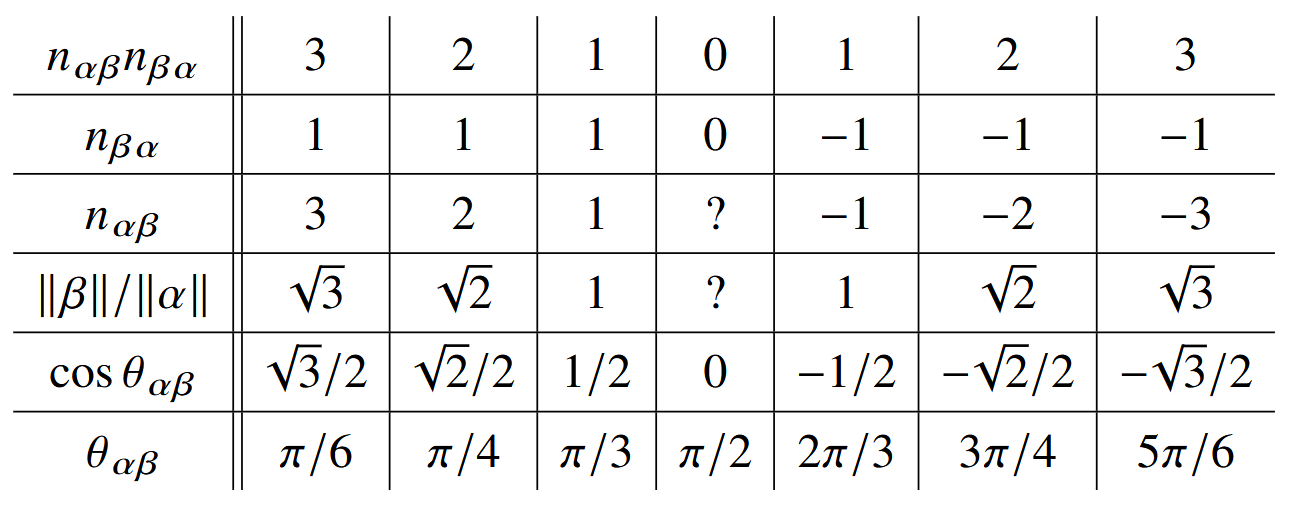
\includegraphics[width=0.8\textwidth]{img/roots-table.png}
    \end{figure}
\end{frame}